\chapter{Erste Standardmodelle der WTheorie} %TODO maybe a chapter have to see

%\subsection{Diskrete Verteilungen}
\section*{Diskrete Verteilungen}

\section{Diskrete Gleichverteilungen}

%TODO restructure! looks like this is just a new section in the chapter Grundbegriffe der WTheorie!
% I think that should be a new chapter, but I am not sure what to do with the unnumbered heading "Diskrete Verteilungen", especially headings "Diskrete Gleichverteilungen" and "Urnenmodelle" should have numbers 2.1 and 2.2 (so should be sections)

Erinnerung:
\begin{definition} %TODO def 1.10?!
	Ist $\Omega$ endlich, so heißt WMaß mit Zähldichte
	\begin{align}
		\rho(\omega) = \frac{1}{\omega}\quad, \omega \in \Omega\notag
	\end{align}
	\begriff{(diskrete) Gleichverteilung} auf $\Omega \to U(\Omega)$\notag
\end{definition}

%\begin{repetition}[\propref{1_10}]
%    Ist $\Omega$ endlich, so heißt WMaß mit Zähldichte
%    \begin{align}
%    \rho(\omega) = \frac{1}{\omega}\quad, \omega \in \Omega\notag
%    \end{align}
%    \begriff{(diskrete) Gleichverteilung} auf $\Omega \to U(\Omega)$.
%\end{repetition}

Es gilt das für jedes $A \in \pows(\Omega)$
\begin{align}
	\probp\brackets{A} = \frac{\abs{A}}{\abs{\Omega}} \notag
\end{align}
Anwendungsbeispiele sind faires Würfeln, fairer Münzwurf, Zahlenlotto, ...


\section{Urnenmodelle}

Ein ``Urnenmodell'' ist eine abstrakte Darstellung von Zufallsexperimenten, bei denen zufällig Stichproben aus einer gegebenen Menge ``gezogen'' werden.
\begin{*definition}[Urne]
	Eine Urne ist ein Behältnis in welchem sich farbige/nummerierte Kugeln befinden, die ansonsten ununterscheidbar sind.
\end{*definition}
Aus der Urne ziehe man blind/zufällig eine oder mehrere Kugeln und notiere Farbe/Zahl.

\begin{center}
    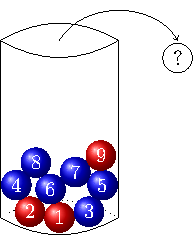
\includegraphics{../../Material/urne_mit_kugeln.pdf}
\end{center}

\subsection{Urnenmodell mit Zurücklegen: Multinomial-Verteilung}

Gegeben: Urne mit $N$ Kugeln, verschiedenfarbig mit Farben aus $E$, $\abs{E} \ge 2$ 

Ziehe: $n$ Stichproben/Kugeln, wobei nach jedem Zug die Kugel wieder zurückgelegt wird. Uns interessiert die Farbe in jedem Zug, setze also
\begin{align}
	\Omega = E^n \und \sigF = \pows(\Omega) \notag
\end{align}
Zur Bestimmung einer geeigneten WMaßes, nummerieren wir die Kugeln mit $1,\dots, N$, so dass alle Kugeln der Farbe $a \in E$ eine Nummer aus $F_{a} \subset \set{1,\dots, N}$ tragen. Würden wir die Nummern notieren, so wäre
\begin{align}
	\overline{\Omega} = \set{1,\dots, N}^n \und \overline{\sigF} = \pows(\overline{\Omega})\notag
\end{align}
und wir könnten die Gleichverteilung $\overline{\probp} = U(\overline{\Omega})$ als WMaß für einem einzelnen Zug verwenden. Für den Übergang zu $\Omega$ konstruieren wir  Zufallsvariablen. Die Farbe im $i$-ten Zug wird beschrieben durch
\begin{align}
	X_i: \overline{\Omega} \to E \mit \overline{\omega} = \left( \overline{\omega}_1, \dots, \overline{\omega}_n \right) \mapsto a \text{ falls } \overline{\omega}_i \in F_a\notag
\end{align}
Der Zufallsvektor
\begin{align}
	X = (X_1, \dots, X_n): \overline{\Omega} \to \Omega\notag
\end{align}
beschreibt dann die Abfolge der Farben. Für jedes $\omega \in \Omega$ gilt dann
\begin{align}
	\set{X = \omega} = F_{\omega_1} \times \cdots \times F_{\omega_n} = \bigtimes_{i=1}^{n} F_{\omega_i}\notag
\end{align}
und damit
\begin{align}
	\probp(\set{\omega}) 
	&= \overline{\probp}(X^{-1}(\set{\omega})) = \probp(X=\omega)\notag\\
	&= \frac{\abs{F_{\omega_1}} \cdots \abs{F_{\omega_n}}}{\abs{\overline{\Omega}}}\notag\\
	&= \prod_{i=1}^{n} \frac{\abs{F_{\omega_i}}}{N} =: \prod_{i=1}^{n} \rho(\omega_i)\notag
\end{align}
Zähldichten, die sich als Produkt von Zähldichten schreiben lassen, werden auch als \begriff{Produktdichten} bezeichnet ($\nearrow$  \S 3 Unabhängigkeit). %TODO ref?!?!?!

Sehr oft interessiert bei einem Urnenexperiment nicht die Reihenfolge der gezogenen Farben, sondern nur die Anzahl der Kugeln in Farbe $a \in E$ nach $n$ Zügen. Dies enspricht
\begin{align}
	 \hat{\Omega} 
	 = \set{k = (k_a)_{a \in E} \in \N_{0}^{\abs{E}} \colon \sum_{a \in E} k_a = n}
	 \und \hat{\sigF} = \pows\brackets{\hat{\Omega}}\notag
\end{align}
Den Übergang $\Omega \to \hat{\Omega}$ beschreiben wir durch die Zufallsvariablen
\begin{align}
	Y_a(\omega): \Omega \to \N_{0} \mit \omega = (\omega_1,\dots, \omega_n)\mapsto \sum_{a \in E} \indi_{\set{a}}(\omega_i)\notag
\end{align}
und
\begin{align}
	Y = \brackets{Y_a}_{a\in E}: \Omega \to \hat{\Omega}\notag
\end{align}

% % % % % % % % % % % % % % % % % % % % 4th lecture % % % % % % % % % % % % % % % % % % % % % % %